% Options for packages loaded elsewhere
% Options for packages loaded elsewhere
\PassOptionsToPackage{unicode}{hyperref}
\PassOptionsToPackage{hyphens}{url}
%
\documentclass[
  ignorenonframetext,
  aspectratio=169,
  russian,
]{beamer}
\newif\ifbibliography
\usepackage{pgfpages}
\setbeamertemplate{caption}[numbered]
\setbeamertemplate{caption label separator}{: }
\setbeamercolor{caption name}{fg=normal text.fg}
\beamertemplatenavigationsymbolshorizontal
% remove section numbering
\setbeamertemplate{part page}{
  \centering
  \begin{beamercolorbox}[sep=16pt,center]{part title}
    \usebeamerfont{part title}\insertpart\par
  \end{beamercolorbox}
}
\setbeamertemplate{section page}{
  \centering
  \begin{beamercolorbox}[sep=12pt,center]{section title}
    \usebeamerfont{section title}\insertsection\par
  \end{beamercolorbox}
}
\setbeamertemplate{subsection page}{
  \centering
  \begin{beamercolorbox}[sep=8pt,center]{subsection title}
    \usebeamerfont{subsection title}\insertsubsection\par
  \end{beamercolorbox}
}
% Prevent slide breaks in the middle of a paragraph
\widowpenalties 1 10000
\raggedbottom
\AtBeginPart{
  \frame{\partpage}
}
\AtBeginSection{
  \ifbibliography
  \else
    \frame{\sectionpage}
  \fi
}
\AtBeginSubsection{
  \frame{\subsectionpage}
}
\usepackage{iftex}
\ifPDFTeX
  \usepackage[T1]{fontenc}
  \usepackage[utf8]{inputenc}
  \usepackage{textcomp} % provide euro and other symbols
\else % if luatex or xetex
  \usepackage{unicode-math} % this also loads fontspec
  \defaultfontfeatures{Scale=MatchLowercase}
  \defaultfontfeatures[\rmfamily]{Ligatures=TeX,Scale=1}
\fi
\usepackage{lmodern}

\ifPDFTeX\else
  % xetex/luatex font selection
\fi
% Use upquote if available, for straight quotes in verbatim environments
\IfFileExists{upquote.sty}{\usepackage{upquote}}{}
\IfFileExists{microtype.sty}{% use microtype if available
  \usepackage[]{microtype}
  \UseMicrotypeSet[protrusion]{basicmath} % disable protrusion for tt fonts
}{}


\usepackage{longtable,booktabs,array}
\usepackage{calc} % for calculating minipage widths
\usepackage{caption}
% Make caption package work with longtable
\makeatletter
\def\fnum@table{\tablename~\thetable}
\makeatother
\usepackage{graphicx}
\makeatletter
\newsavebox\pandoc@box
\newcommand*\pandocbounded[1]{% scales image to fit in text height/width
  \sbox\pandoc@box{#1}%
  \Gscale@div\@tempa{\textheight}{\dimexpr\ht\pandoc@box+\dp\pandoc@box\relax}%
  \Gscale@div\@tempb{\linewidth}{\wd\pandoc@box}%
  \ifdim\@tempb\p@<\@tempa\p@\let\@tempa\@tempb\fi% select the smaller of both
  \ifdim\@tempa\p@<\p@\scalebox{\@tempa}{\usebox\pandoc@box}%
  \else\usebox{\pandoc@box}%
  \fi%
}
% Set default figure placement to htbp
\def\fps@figure{htbp}
\makeatother



\ifLuaTeX
\usepackage[bidi=basic,provide=*]{babel}
\else
\usepackage[bidi=default,provide=*]{babel}
\fi
% get rid of language-specific shorthands (see #6817):
\let\LanguageShortHands\languageshorthands
\def\languageshorthands#1{}


\setlength{\emergencystretch}{3em} % prevent overfull lines

\providecommand{\tightlist}{%
  \setlength{\itemsep}{0pt}\setlength{\parskip}{0pt}}



 

\usepackage[]{csquotes}

\IfFileExists{plex-otf.sty}{
  %% Full TeXlive
  % \usepackage[%
  %   % math,
  %   RM={Scale=0.94},SS={Scale=0.94},SScon={Scale=0.94},TT={Scale=MatchLowercase,FakeStretch=0.9},DefaultFeatures={Ligatures=Common}
  % ]{plex-otf}
}{
  %% TinyTeX
  \usepackage{libertine}
}

%%% Load theme
% https://deic.uab.cat/~iblanes/beamer_gallery/
\IfFileExists{beamerthemegotham.sty}{
  %% Full TeXlive
  \usetheme{gotham}
  \gothamset{
    numbering=totalpagenumber,
    parttocframe default=off,
    sectiontocframe default=off,
    subsectiontocframe default=off,
  }
}{
  %% TinyTeX
  \usetheme{Madrid}
}
\makeatletter
\@ifpackageloaded{caption}{}{\usepackage{caption}}
\AtBeginDocument{%
\ifdefined\contentsname
  \renewcommand*\contentsname{Содержание}
\else
  \newcommand\contentsname{Содержание}
\fi
\ifdefined\listfigurename
  \renewcommand*\listfigurename{Список иллюстраций}
\else
  \newcommand\listfigurename{Список иллюстраций}
\fi
\ifdefined\listtablename
  \renewcommand*\listtablename{Список таблиц}
\else
  \newcommand\listtablename{Список таблиц}
\fi
\ifdefined\figurename
  \renewcommand*\figurename{Рисунок}
\else
  \newcommand\figurename{Рисунок}
\fi
\ifdefined\tablename
  \renewcommand*\tablename{Таблица}
\else
  \newcommand\tablename{Таблица}
\fi
}
\@ifpackageloaded{float}{}{\usepackage{float}}
\floatstyle{ruled}
\@ifundefined{c@chapter}{\newfloat{codelisting}{h}{lop}}{\newfloat{codelisting}{h}{lop}[chapter]}
\floatname{codelisting}{Список}
\newcommand*\listoflistings{\listof{codelisting}{Листинги}}
\makeatother
\makeatletter
\makeatother
\makeatletter
\@ifpackageloaded{caption}{}{\usepackage{caption}}
\@ifpackageloaded{subcaption}{}{\usepackage{subcaption}}
\makeatother

\usepackage{bookmark}
\IfFileExists{xurl.sty}{\usepackage{xurl}}{} % add URL line breaks if available
\urlstyle{same}
\hypersetup{
  pdftitle={Механизмы SetUID, SetGID и Sticky-битов в Linux},
  pdfauthor={Алексей Прядко},
  pdflang={ru-RU},
  hidelinks,
  pdfcreator={LaTeX via pandoc}}


\title{Механизмы SetUID, SetGID и Sticky-битов в Linux}
\subtitle{Лабораторная работа №5}
\author{Алексей Прядко}
\date{2026-04-18}

\begin{document}
\frame{\titlepage}

\renewcommand*\contentsname{Содержание}
\begin{frame}[allowframebreaks]
  \frametitle{Содержание}
  \setcounter{tocdepth}{1}
  \tableofcontents
\end{frame}
\setcounter{tocdepth}{1}
\tableofcontents
}

\section{Информация}\label{ux438ux43dux444ux43eux440ux43cux430ux446ux438ux44f}

\begin{frame}{Докладчик}
\phantomsection\label{ux434ux43eux43aux43bux430ux434ux447ux438ux43a}
\begin{columns}[c]
\begin{column}{0.7\linewidth}
\begin{itemize}[<+->]
\tightlist
\item
  Алексей Прядко
\item
  НБИбд-01-24
\item
  Кафедра информационной безопасности
\end{itemize}
\end{column}

\begin{column}{0.3\linewidth}
\end{column}
\end{columns}
\end{frame}

\section{Вводная
часть}\label{ux432ux432ux43eux434ux43dux430ux44f-ux447ux430ux441ux442ux44c}

\begin{frame}{Актуальность}
\phantomsection\label{ux430ux43aux442ux443ux430ux43bux44cux43dux43eux441ux442ux44c}
\begin{itemize}[<+->]
\tightlist
\item
  В Linux права доступа --- основа безопасности
\item
  SetUID и SetGID позволяют процессам временно повышать привилегии
\item
  Sticky-бит защищает общие каталоги от случайного удаления файлов
\item
  Понимание этих механизмов необходимо администраторам и специалистам по
  ИБ
\end{itemize}
\end{frame}

\begin{frame}{Объект и предмет исследования}
\phantomsection\label{ux43eux431ux44aux435ux43aux442-ux438-ux43fux440ux435ux434ux43cux435ux442-ux438ux441ux441ux43bux435ux434ux43eux432ux430ux43dux438ux44f}
\begin{itemize}[<+->]
\tightlist
\item
  Объект: файловая система Linux с расширенными атрибутами
\item
  Предмет: поведение процессов при наличии SetUID/SetGID-битов и влияние
  Sticky-бита на операции с файлами
\end{itemize}
\end{frame}

\begin{frame}[fragile]{Цели и задачи}
\phantomsection\label{ux446ux435ux43bux438-ux438-ux437ux430ux434ux430ux447ux438}
\textbf{Цель:} изучить механизмы изменения идентификаторов процессов и
влияние Sticky-бита.

\textbf{Задачи:} 1. Написать программы для отображения UID/GID 2.
Исследовать SetUID и SetGID на примере 3. Проверить возможность чтения
защищённого файла через SetUID 4. Изучить работу Sticky-бита на каталоге
\texttt{/tmp}
\end{frame}

\begin{frame}[fragile]{Материалы и методы}
\phantomsection\label{ux43cux430ux442ux435ux440ux438ux430ux43bux44b-ux438-ux43cux435ux442ux43eux434ux44b}
\begin{itemize}[<+->]
\tightlist
\item
  ОС Rocky Linux 8.10
\item
  Компилятор GCC, текстовый редактор nano
\item
  Работа в терминале от разных пользователей
\item
  Команды \texttt{chmod}, \texttt{chown}, \texttt{ls}, \texttt{su}
\end{itemize}
\end{frame}

\section{Ход выполнения
работы}\label{ux445ux43eux434-ux432ux44bux43fux43eux43bux43dux435ux43dux438ux44f-ux440ux430ux431ux43eux442ux44b}

\begin{frame}[fragile]{Подготовка стенда}
\phantomsection\label{ux43fux43eux434ux433ux43eux442ux43eux432ux43aux430-ux441ux442ux435ux43dux434ux430}
\begin{itemize}[<+->]
\tightlist
\item
  Проверка наличия GCC: \texttt{gcc\ -\/-version}
\item
  Отключение SELinux: \texttt{setenforce\ 0}
\item
  Создание пользователя \texttt{guest2} (использован существующий
  \texttt{guest})
\end{itemize}

\begin{figure}[H]

{\centering 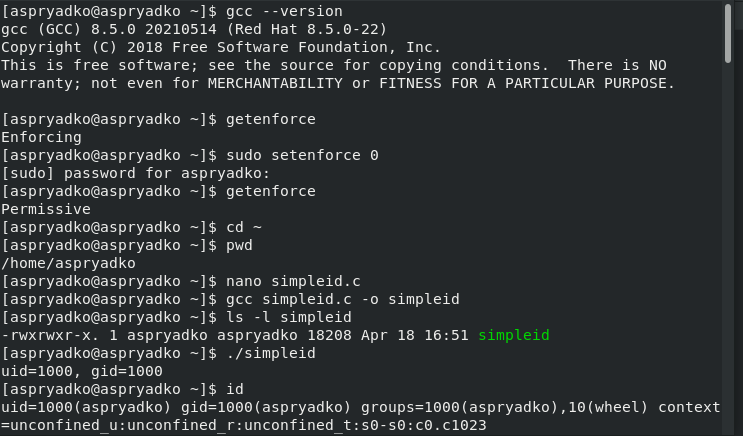
\includegraphics[width=0.9\linewidth,height=\textheight,keepaspectratio]{image/01_prepare_and_simpleid.png}

}

\caption{Подготовка стенда}

\end{figure}%
\end{frame}

\begin{frame}[fragile]{Программа simpleid и реальные ID}
\phantomsection\label{ux43fux440ux43eux433ux440ux430ux43cux43cux430-simpleid-ux438-ux440ux435ux430ux43bux44cux43dux44bux435-id}
\begin{itemize}[<+->]
\tightlist
\item
  Создан \texttt{simpleid.c}, выводящий \texttt{uid} и \texttt{gid}
\item
  Результат совпадает с командой \texttt{id}
\item
  Пользователь \texttt{aspryadko} → UID=1000, GID=1000
\end{itemize}

\begin{figure}[H]

{\centering 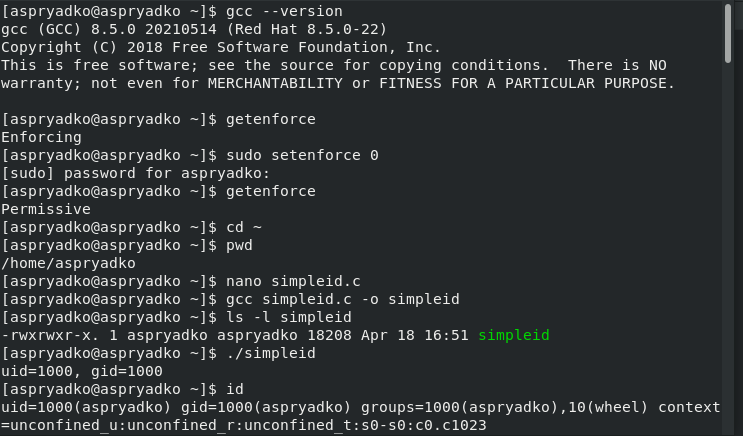
\includegraphics[width=0.7\linewidth,height=\textheight,keepaspectratio]{image/01_prepare_and_simpleid.png}

}

\caption{simpleid}

\end{figure}%
\end{frame}

\begin{frame}[fragile]{Программа simpleid2: реальные и эффективные ID}
\phantomsection\label{ux43fux440ux43eux433ux440ux430ux43cux43cux430-simpleid2-ux440ux435ux430ux43bux44cux43dux44bux435-ux438-ux44dux444ux444ux435ux43aux442ux438ux432ux43dux44bux435-id}
\begin{itemize}[<+->]
\tightlist
\item
  Добавлены \texttt{getuid()/geteuid()}, \texttt{getgid()/getegid()}
\item
  Изначально реальные и эффективные ID совпадают
\item
  После установки SetUID (владелец root) эффективный UID становится 0
\end{itemize}

\begin{figure}[H]

{\centering 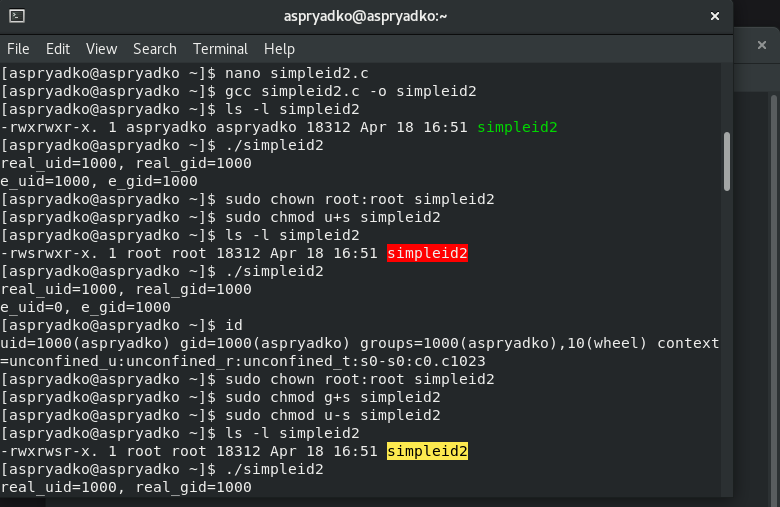
\includegraphics[width=0.9\linewidth,height=\textheight,keepaspectratio]{image/02_setuid_simpleid2.png}

}

\caption{SetUID}

\end{figure}%
\end{frame}

\begin{frame}{Исследование SetGID}
\phantomsection\label{ux438ux441ux441ux43bux435ux434ux43eux432ux430ux43dux438ux435-setgid}
\begin{itemize}[<+->]
\tightlist
\item
  SetUID снят, установлен SetGID
\item
  Группа-владелец остаётся root
\item
  Эффективный GID становится 0, UID возвращается к 1000
\end{itemize}

\begin{figure}[H]

{\centering 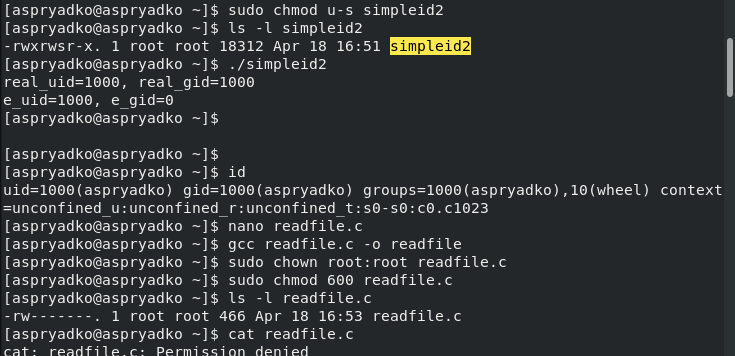
\includegraphics[width=0.9\linewidth,height=\textheight,keepaspectratio]{image/03_setgid_simpleid2.png}

}

\caption{SetGID}

\end{figure}%
\end{frame}

\begin{frame}[fragile]{Программа readfile: доступ к защищённому файлу}
\phantomsection\label{ux43fux440ux43eux433ux440ux430ux43cux43cux430-readfile-ux434ux43eux441ux442ux443ux43f-ux43a-ux437ux430ux449ux438ux449ux451ux43dux43dux43eux43cux443-ux444ux430ux439ux43bux443}
\begin{itemize}[<+->]
\tightlist
\item
  Программа читает любой файл, переданный аргументом
\item
  Файл \texttt{readfile.c} защищён (\texttt{600}, владелец root)
\item
  Обычный пользователь не может прочитать (\texttt{Permission\ denied})
\item
  После установки SetUID на \texttt{readfile} программа читает и
  \texttt{readfile.c}, и \texttt{/etc/shadow}
\end{itemize}

\begin{figure}[H]

{\centering 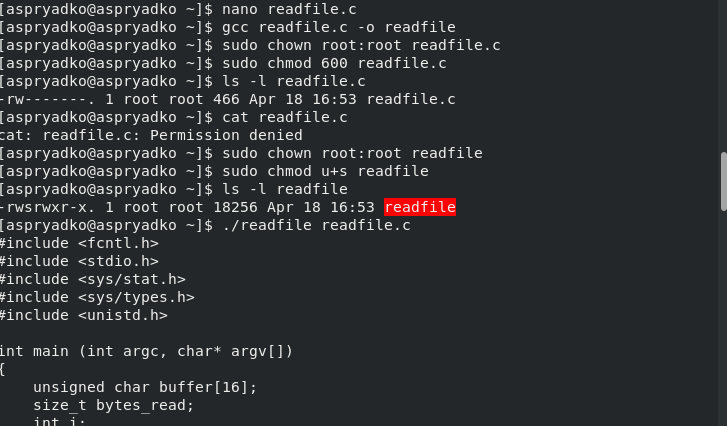
\includegraphics[width=0.9\linewidth,height=\textheight,keepaspectratio]{image/04_readfile_setuid.png}

}

\caption{readfile SetUID}

\end{figure}%
\end{frame}

\begin{frame}[fragile]{Sticky-бит на \texttt{/tmp}: проверка при
включённом t}
\phantomsection\label{sticky-ux431ux438ux442-ux43dux430-tmp-ux43fux440ux43eux432ux435ux440ux43aux430-ux43fux440ux438-ux432ux43aux43bux44eux447ux451ux43dux43dux43eux43c-t}
\begin{itemize}[<+->]
\tightlist
\item
  \texttt{/tmp} имеет бит \texttt{t} (\texttt{drwxrwxrwt})
\item
  Файл создан пользователем \texttt{aspryadko}, права \texttt{o+rw}
\item
  Пользователь \texttt{guest} может читать, дописывать, перезаписывать
\item
  Удалить файл \textbf{не может} (\texttt{Operation\ not\ permitted})
\end{itemize}

\begin{figure}[H]

{\centering 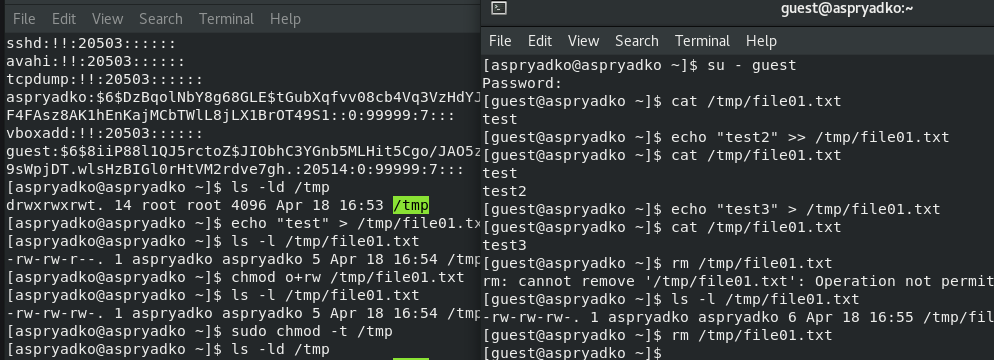
\includegraphics[width=0.9\linewidth,height=\textheight,keepaspectratio]{image/05_sticky_enabled.png}

}

\caption{Sticky enabled}

\end{figure}%
\end{frame}

\begin{frame}[fragile]{Sticky-бит на \texttt{/tmp}: после снятия t}
\phantomsection\label{sticky-ux431ux438ux442-ux43dux430-tmp-ux43fux43eux441ux43bux435-ux441ux43dux44fux442ux438ux44f-t}
\begin{itemize}[<+->]
\tightlist
\item
  Команда \texttt{sudo\ chmod\ -t\ /tmp} убирает бит
\item
  Пользователь \texttt{guest} успешно удаляет файл
\item
  Возврат бита: \texttt{sudo\ chmod\ +t\ /tmp}
\end{itemize}

\begin{figure}[H]

{\centering 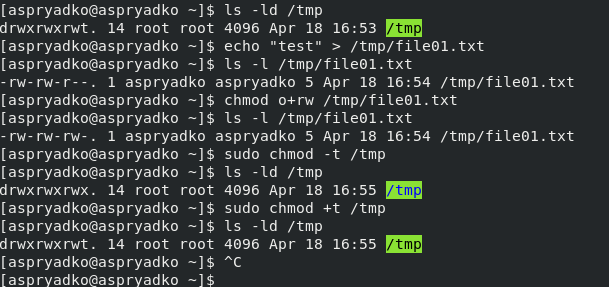
\includegraphics[width=0.9\linewidth,height=\textheight,keepaspectratio]{image/06_sticky_disabled.png}

}

\caption{Sticky disabled}

\end{figure}%
\end{frame}

\section{Результаты}\label{ux440ux435ux437ux443ux43bux44cux442ux430ux442ux44b}

\begin{frame}[fragile]{Основные выводы}
\phantomsection\label{ux43eux441ux43dux43eux432ux43dux44bux435-ux432ux44bux432ux43eux434ux44b}
\begin{itemize}[<+->]
\tightlist
\item
  \textbf{SetUID} изменяет эффективный UID на владельца файла, что
  позволяет временно повысить привилегии
\item
  \textbf{SetGID} аналогично действует на эффективный GID
\item
  Программа с SetUID от root может читать защищённые файлы (например,
  \texttt{/etc/shadow})
\item
  \textbf{Sticky-бит} защищает файлы в общих каталогах от удаления
  посторонними пользователями
\end{itemize}
\end{frame}

\begin{frame}{Практическая значимость}
\phantomsection\label{ux43fux440ux430ux43aux442ux438ux447ux435ux441ux43aux430ux44f-ux437ux43dux430ux447ux438ux43cux43eux441ux442ux44c}
\begin{itemize}[<+->]
\tightlist
\item
  Получены навыки управления расширенными атрибутами файлов
\item
  Понимание этих механизмов необходимо для настройки безопасной среды в
  Linux
\item
  Осознаны риски неправильного использования SetUID
\end{itemize}
\end{frame}

\section{Заключение}\label{ux437ux430ux43aux43bux44eux447ux435ux43dux438ux435}

\begin{frame}{Итоги}
\phantomsection\label{ux438ux442ux43eux433ux438}
\begin{itemize}[<+->]
\tightlist
\item
  Лабораторная работа выполнена в полном объёме
\item
  Изучены SetUID, SetGID и Sticky-биты
\item
  Результаты подтверждены скриншотами
\item
  Полученные знания применимы в администрировании и информационной
  безопасности
\end{itemize}
\end{frame}

\begin{frame}{Спасибо за внимание!}
\phantomsection\label{ux441ux43fux430ux441ux438ux431ux43e-ux437ux430-ux432ux43dux438ux43cux430ux43dux438ux435}
\end{frame}




\end{document}
